\chapter{Qubit Mapping Illustration} \label{app:virtual-on-physical-illustration}
\begin{figure}[!htb]
    \centering
    \begin{subfigure}{0.3\linewidth}
        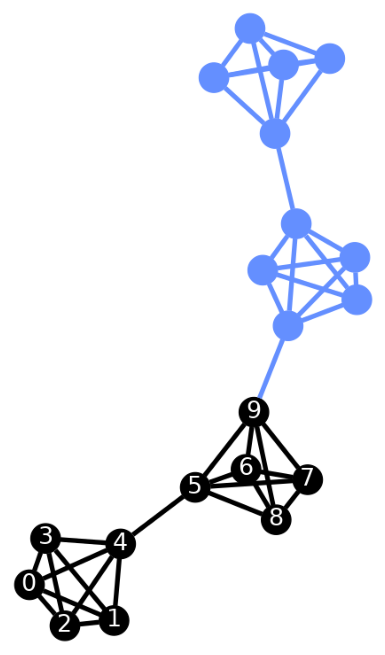
\includegraphics[width=\linewidth]{image/dj_10_full_5_4.png}
        \caption{full\_5\_4 layout}
        \label{fig:dj_10_full_5_4}
    \end{subfigure}
    \hfill
    \begin{subfigure}{0.3\linewidth}
        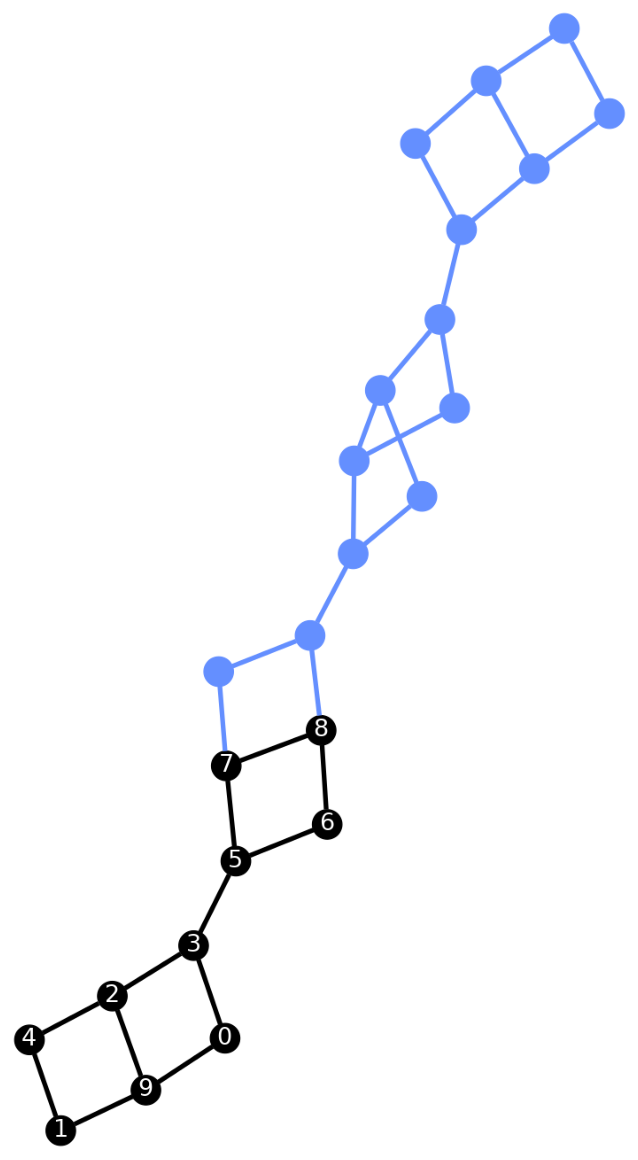
\includegraphics[width=\linewidth]{image/dj_10_grid_6_4.png}
        \caption{grid\_6\_4 layout}
        \label{fig:dj_10_grid_6_4}
    \end{subfigure}
    \hfill
    \begin{subfigure}{0.3\linewidth}
        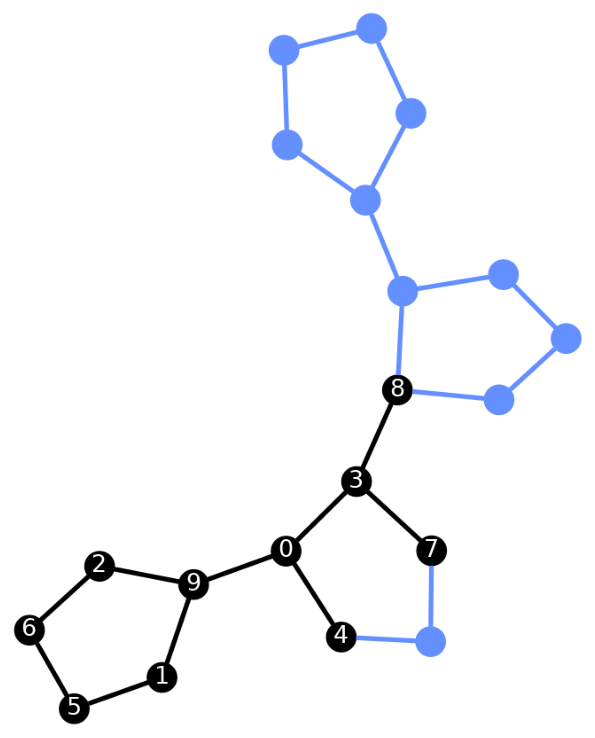
\includegraphics[width=\linewidth]{image/dj_10_ring_5_4.png}
        \caption{ring\_5\_4 layout}
        \label{fig:dj_10_ring_5_4}
    \end{subfigure}
    \hfill
    \begin{subfigure}{0.25\linewidth}
        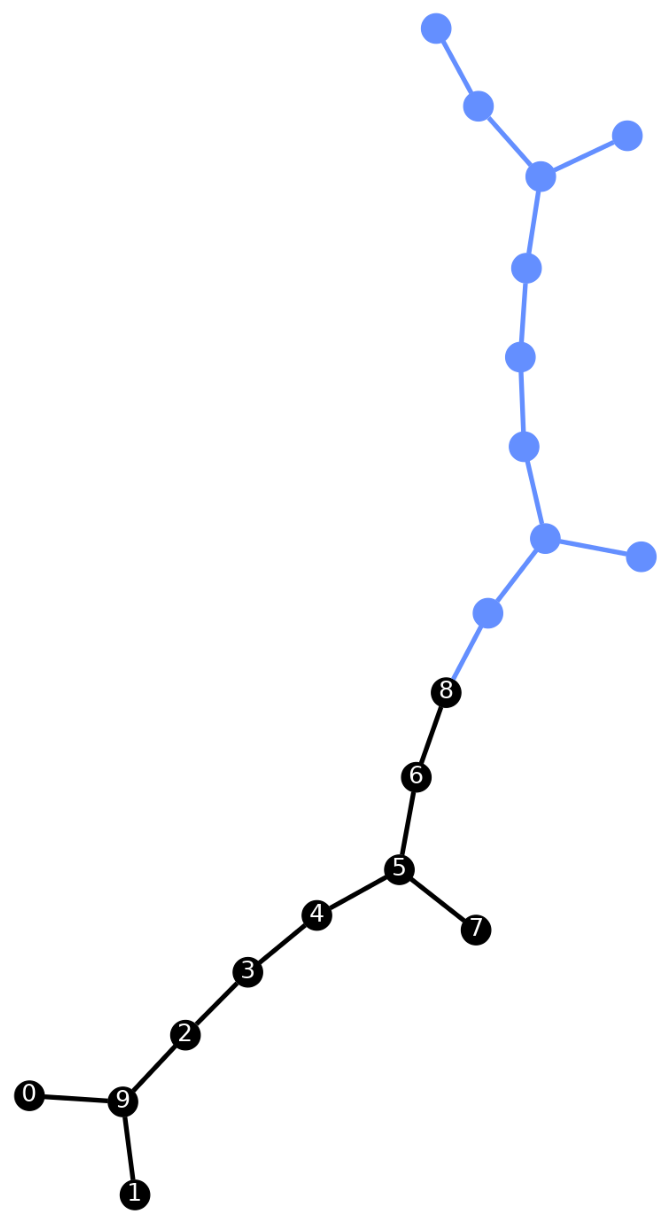
\includegraphics[width=\linewidth]{image/dj_10_t_horizontal_5_4.png}
        \caption{t\_horizontal\_5\_4 layout}
        \label{fig:dj_10_t_horizontal_5_4}
    \end{subfigure}
    \hfill
    \begin{subfigure}{0.25\linewidth}
        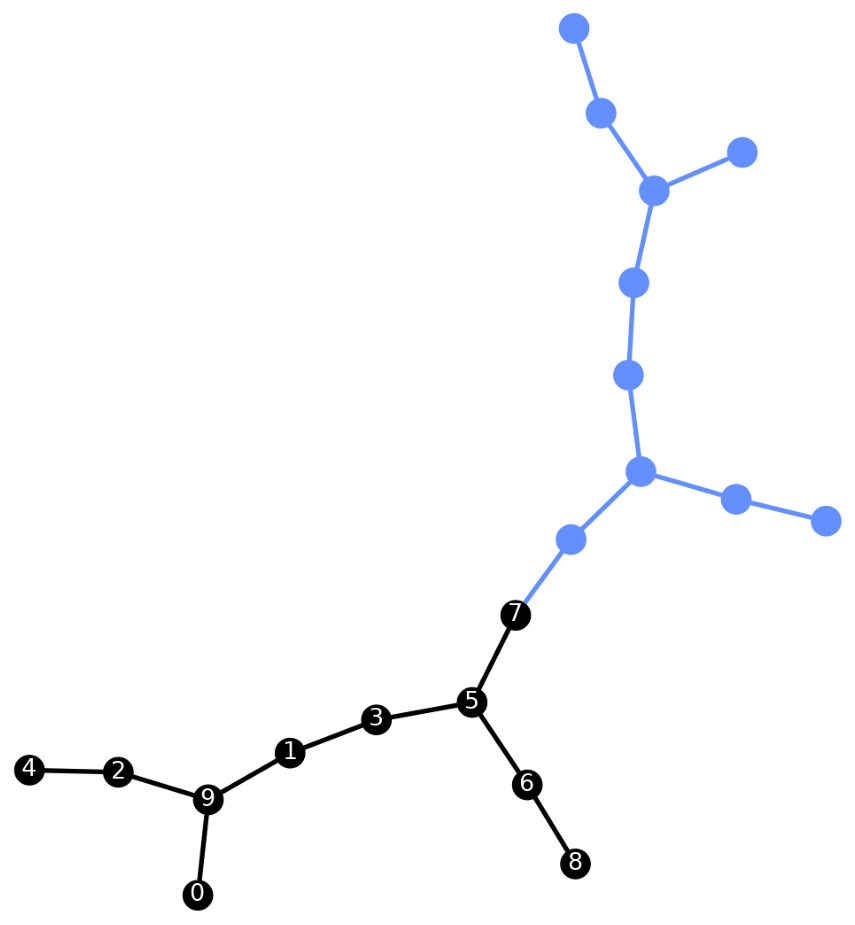
\includegraphics[width=\linewidth]{image/dj_10_t_vertical_5_4.png}
        \caption{t\_horizontal\_5\_4 layout}
        \label{fig:dj_10_t_vertical_5_4}
    \end{subfigure}
    \caption{Deutsch-Jozsa n = 10 in coupling map. Black nodes with numbers illustrate the location of logical qubits, and blue nodes illustrate the available physical qubits.}
    \label{fig:dj-10-layout}
\end{figure}